\documentclass[class=book, crop=false, oneside, 12pt]{standalone}
\usepackage{standalone}
\usepackage{amsmath}
\usepackage{../../style}
\graphicspath{{./assets/images/}}

% arara: pdflatex: { synctex: yes, shell: yes }
% arara: latexmk: { clean: partial }
\begin{document}

\chapter{Conduttori, dielettrici, energia elettrostatica}

\section{Conduttori in equilibrio}

\subsection{Condizione di equilibrio per un conduttore}

I materiali conduttori sono caratterizzati dal fatto che nel loro interno sono verificate particolari condizioni per cui è possibile il moto di alcune delle cariche che li costituiscono.  
La nostra trattazione si concentra sui conduttori solidi, il cui esempio più tipico sono i metalli: in essi per ogni atomo si hanno uno o più elettroni che sono in pratica separati dal resto dell'atomo e liberi di muoversi nel conduttore. 
Con l'applicazione di un opportuno campo \(\overrightarrow{E}\) si può provocare un moto ordinato di elettroni ovvero dar luogo a una corrente elettrica.

Nei fenomeni elettrostatici però le cariche sono fisse e questa condizione richiede che all'interno di un conduttore il campo debba essere nullo, altrimenti ci sarebbe un moto di cariche, contrariamente all'ipotesi. 
Pertanto lo stato di conduttore in \emph{equilibrio elettrostatico} è definito dalla condizione: 
\begin{equation*}
    \overrightarrow{E} = 0 \text{ all'interno }
\end{equation*}
Si deve intendere che questa è una condizione media macroscopica. 
Nelle immediate vicinanze dei nuclei ci sono campi molto intensi che tengono legati gli elettroni non liberi; inoltre gli elettroni liberi non sono in quiete ma hanno un moto completamente disordinato di agitazione termica. 
Però in nessun istante c'è un moto ordinato in una certa direzione degli elettroni liberi rispetto agli ioni metallici fissi; si usa per questo parlare di gas di elettroni liberi all'interno di un conduttore.

La condizione \(\overrightarrow{E} = 0\) ha le seguenti conseguenze che caratterizzano un conduttore in equilibrio elettrostatico: 
\begin{itemize}
    \item l'eccesso di carica elettrica in un conduttore può stare solo sulla superficie del conduttore;
    \item il potenziale elettrostatico è costante su tutto il conduttore;
    \item il campo elettrostatico in un punto delle vicinanze della superficie del conduttore è perpendicolare alla superficie e ha intensità \(\sigma/ \epsilon_0\), con \(\sigma\) densità di carica superficiale in quel punto.
\end{itemize}
Per la prima proprietà, se il campo elettrostatico è nullo, è nullo il flusso attraverso una qualunque superficie chiusa \(\Sigma^{\prime}\) tracciata all'interno del conduttore e quindi secondo la legge di Gauss all'interno del conduttore non ci sono cariche ( \(q_{int} = 0\)).
Pertanto l'eccesso di carica si distribuisce sulla superficie del conduttore con densità superficiale \(\sigma = dq/ d \Sigma\); se si cedono al conduttore elettroni questi si portano sulla superficie, se si sottraggono, ne risulta carente lo strato superficiale. 

Il potenziale elettrostatico risulta costante in ogni punto del conduttore perché presi due punti qualsiasi
\begin{equation*}
    V(P_2) - V(P_1) = - \int_{P_1}^{P_2} \overrightarrow{E} \cdot d \overrightarrow{s} = 0 \implies V(P_2) = V(P_1) = V_0
\end{equation*}
Il risultato è vero anche se uno dei due punti sta sulla superficie del conduttore, che risulta quindi essere una \emph{superficie equipotenziale}. 

\subsection{Teorema di Coulomb}

Dato che la superficie del conduttore è equipotenziale, il campo elettrostatico \(\overrightarrow{E}\) in un punto esterno molto vicino al conduttore è ortogonale alla superficie del conduttore, indipendentemente dalla forma di questo.

Il valore di \(\overrightarrow{E}\) si ricava applicando la legge di Gauss ad un cilindro retto di basi \(d \Sigma\) e superficie laterale di area trascurabile rispetto a \(d \Sigma\), con una base contenuta all'interno del conduttore, in cui \(E = 0\), e l'altra in prossimità immediata del conduttore all'esterno, dove il campo elettrostatico \(\overrightarrow{E}\) è normale alla superficie. 
Detta \(dq\) la carica contenuta all'interno, sulla superficie del conduttore, si ha:
\begin{equation*}
    \oint \overrightarrow{E} \cdot \overrightarrow{u}_n d \Sigma = E d \Sigma = \frac{1}{\epsilon_0} d q = \frac{1}{\epsilon_0} \sigma d \Sigma
\end{equation*}
e quindi
\begin{equation} \label{teorema_coulomb}
    \overrightarrow{E} = \frac{\sigma}{\epsilon_0}\overrightarrow{u}_n
\end{equation}
\begin{figure}[h]
    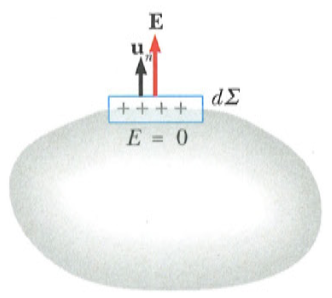
\includegraphics[scale=0.4]{conduttore_campo.png}
    \centering
    \caption{}
\end{figure}
detto anche \emph{Teorema di Coulomb}. 
Il verso è \emph{uscente} se la densità è \emph{positiva}, \emph{entrante} se è \emph{negativa}. 
Si vede che il modulo del campo elettrostatico è maggiore dove \(\sigma\) è maggiore (questo avviene dove il raggio di curvatura è minore).

Un conduttore carico \emph{lontano da altri conduttori} ha dunque una distribuzione superficiale di carica tale che il campo elettrostatico all'interno sia nullo, qualunque sia la forma del conduttore. 
In particolare se il conduttore è sferico la carica è distribuita uniformemente.
Notiamo inoltre che la carica deve avere lo stesso segno, positivo o negativo, ovunque sulla superficie: un accumulo di elettroni soltanto in una certa zona sarebbe dovuto esclusivamente a un campo elettrico esterno.

\begin{figure}[h]
    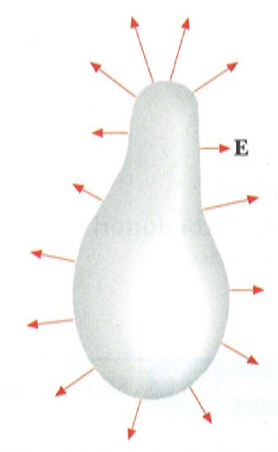
\includegraphics[scale=0.4]{conduttore_linee.png}
    \centering
    \caption{}
\end{figure}

\subsection{Induzione elettrostatica}

Avvicinando un conduttore, carico o scarico, ad un altro corpo carico, ovvero introducendolo in un campo elettrico esterno \(\overrightarrow{E}\), il campo elettrostatico all'interno non sarebbe più nullo, ma sarebbe dato da \(\overrightarrow{E}\); senonché questo fatto provoca un movimento di elettroni che si spostano per l'azione del campo elettrico esterno e si accumulano in una zona della superficie, lasciando sul resto della superficie un eccesso di carica positiva: 
tra queste zone si crea un campo dettrostatico indotto \(\overrightarrow{E}_i\) che contrasta il movimento degli elettroni e si raggiunge l'equilibrio quando \(E + E_i = 0\) in tutto l'interno del conduttore.
Abbiamo così una distribuzione di carica elettrica indotta dei due segni sulla superficie del conduttore che si sovrappone all'eventuale carica elettrica preesistente; in totale però la carica elettrica del conduttore rimane la stessa poiché la carica elettrica indotta è la somma algebrica dei due contributi eguali ed opposti.
È il caso dell'induzione elettrostatica.

Se poniamo a contatto due o più conduttori, ad esempio collegandoli con un filo conduttore, si costituisce un unico corpo conduttore e in equilibrio vale ovunque la condizione \(E = 0\), \(V =\text{ costante}\): i conduttori a contatto hanno lo stesso potenziale. 

\section{Conduttore cavo, schermo elettrostatico}

\subsection{Conduttore cavo}

\begin{figure}[h]
    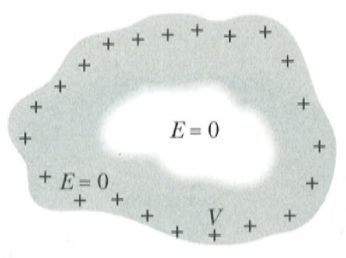
\includegraphics[scale=0.4]{conduttore_cavo.png}
    \centering
    \caption{}
\end{figure}

Consideriamo un conduttore carico che abbia nel suo interno una cavità all'interno della quale non ci siano cariche elettriche. 
Nella massa del conduttore il campo elettrostatico è nullo e pertanto è nullo il flusso attraverso qualsiasi superficie chiusa, in particolare attraverso qualsiasi superficie chiusa \(\Sigma\) che racchiuda la cavità: segue, per la legge di Gauss, che all'interno di \(\Sigma\) non ci sono cariche e quindi sulle pareti della cavità la carica è nulla.

\subsubsection{Dimostrazione}

Se sulle pareti della cavità fossero presenti due distribuzioni di carica di segno opposto, ci sarebbero nella cavità linee di forza, uscenti dalle cariche positive e entranti in quelle negative. 
La circuitazione di \(\overrightarrow{E}\) lungo una linea chiusa, costituita da un tratto \(C_1\) interno alla cavità su cui \(\overrightarrow{E} \neq 0\) e da un tratto \(C_2\) interno al conduttore dove \(\overrightarrow{E} = 0\), darebbe
\begin{equation*}
    \oint \overrightarrow{E} \cdot d \overrightarrow{s} = \int_{C_1} \overrightarrow{E} \cdot d \overrightarrow{s} + \int_{C_2} \overrightarrow{E} \cdot d \overrightarrow{s} = \int_{C_1} \overrightarrow{E} \cdot d \overrightarrow{s} \neq 0
\end{equation*}
in contrasto col fatto che \(\overrightarrow{E}\) è conservativo. 
Pertanto il campo nella cavità deve essere nullo se l'integrale di linea esteso a qualsiasi percorso \(C_1\) interno alla cavità deve essere nullo: sulle pareti della cavità non possono esserci cariche elettriche.
Inoltre è chiaro che il potenziale elettrostatico in un qualsiasi punto della cavità è uguale a quello del conduttore: se ci fosse una differenza di potenziale dovrebbe infatti esserci un campo elettrostatico diverso da zero. 

In conclusione:
\begin{itemize}
    \item la carica di un conduttore in equilibrio elettrostatico si distribuisce sempre e soltanto sulla superficie esterna, anche in presenza di una o più cavità all'interno del conduttore; 
    \item il campo elettrostatico è nullo e il potenziale elettrostatico è costante in ogni punto interno alla superficie del conduttore, anche in presenza di cavità.
\end{itemize}

In particolare un conduttore sferico isolato carico di raggio \(R\), che sia pieno o con una cavità sferica concentrica o con cavità di qualsiasi forma, ha sempre campo elettrostatico nullo all'interno e campo elettrostatico in vicinanza della superficie esterna:
\begin{equation*}
    \overrightarrow{E} = \frac{\sigma}{\epsilon_0} \overrightarrow{u}_n = \frac{q}{4 \pi \epsilon_0 R^2}
\end{equation*}
uguale a quella di una carica puntiforme \(q\) posta nel centro \(O\) della superficie sferica. 

\subsection{Induzione completa}

Consideriamo adesso un conduttore \(C_2\) cavo, isolato e privo di carica, e introduciamo un altro conduttore \(C_1\) carico nella cavità, mantenendolo isolato da \(C_2\). 
In condizioni di equilibrio, se \(C_1\) ha sulla sua superficie esterna una carica \(q\), una carica \(- q\) risulta distribuita sulla superficie interna e una carica \(q\) sulla superficie esterna di \(C_2\).

\begin{figure}[h]
    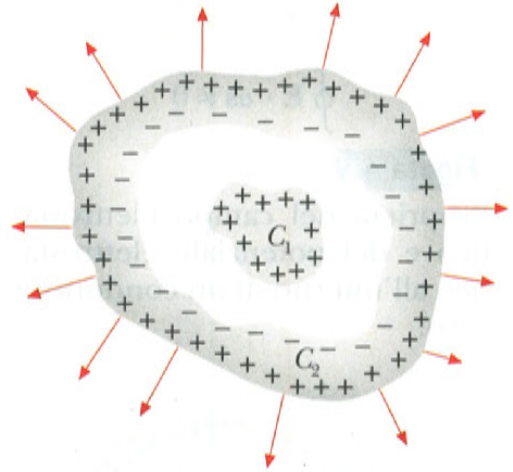
\includegraphics[scale=0.4]{induzione_elettrostatica_completa.png}
    \centering
    \caption{}
\end{figure}

\subsubsection{Dimostrazione}

Tale fatto si spiega subito con la legge di Gauss: attraverso una superficie chiusa \(\Sigma\) interna a \(C_2\) e contenente la cavità il flusso di \(\overrightarrow{E}\) è nullo in quanto è nullo il campo stesso; di conseguenza all'interno di \(\Sigma\) non c'è carica e se \(C_1\) porta la carica \(q\), sulla superficie interna di \(C_2\) deve necessariamente comparire una carica \(-q\). 
Inoltre essendo \(C_2\) neutro, lo spostamento di una carica \(- q\) sulla superficie interna provoca la comparsa di una carica \(+q\) sulla superficie esterna. 

Siamo di fronte a un fenomeno di induzione che in questo caso, essendo la carica \(q\) completamente contenuta all'interno di una cavità chiusa, si chiama induzione completa: \emph{tutte le linee di forza che partono da \(C_1\) terminano su \(C_2\)}.

Dalla superficie esterna di \(C_2\) partono altre linee di forza, il cui andamento in prossimità del conduttore riflette la distribuzione delle cariche sulla superficie stessa. 
Le due zone in cui esiste un campo sono separate da una zona in cui, in equilibrio, non può esistere campo elettrostatico. 

Il campo elettrostatico all'interno della cavità è determinato dal valore di \(q\), dalla posizione di \(C_1\) e dalla forma geometrica delle due superficie affacciate. 
Però, fissato \(q\), all'esterno l'effetto è sempre lo stesso, qualunque siano forma e  posizione. 
Infatti possiamo dire che l'informazione sulla situazione interna potrebbe passàre all'esterno solo attraverso un campo elettrostatico che penetrasse nel conduttore \(C_2\): ma questo non è possibile per la proprietà dei conduttori in equilibrio di avere campo elettrostatico nullo all'interno. 
Al limite si può portare \(C_1\) a contatto con \(C_2\), con il che le cariche \(+q\) e \(-q\) si elidono, ma all'esterno non cambia nulla: questo fatto ci fa anche capire che la distribuzione della carica \(-q\) sulla faccia interna di \(C_2\) è sempre tale che, sommando l'effetto della carica \(q\) di \(C_1\), il campo elettrostatico dovuto alle cariche nella cavità è nullo all'esterno della cavità.

Analogamente, se variamo la carica sulla superficie esterna oppure variamo la sua distribuzione, ad esempio avvicinando al conduttore un altro corpo carico, cambia il campo elettrostatico all'esterno, ma la distribuzione di carica sulla superficie esterna di \(C_2\) è sempre tale da dare campo elettrostatico nullo all'interno di \(C_2\) e quindi non può alterare il campo locale esistente nella cavità. 

\subsection{Schermo elettrostatico}

Pertanto finché lo spazio interno e lo spazio esterno non sono comunicanti: il conduttore cavo costituisce uno schermo elettrostatico perfetto tra spazio interno e spazio esterno

\section{Condensatori}

\begin{figure}[h]
    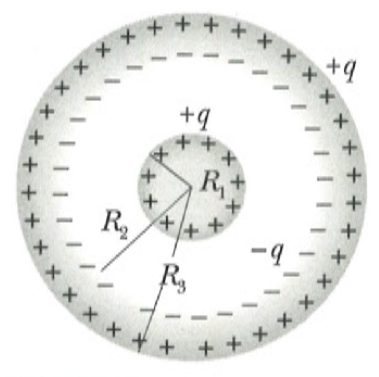
\includegraphics[scale=0.4]{condensatore_sferico.png}
    \centering
    \caption{}
\end{figure}

Consideriamo il sistema costituito da un conduttore sferico di raggio \(R_1\) al centro di un conduttore sferico cavo di raggio interno \(R_2\) e raggio esterno \(R_3\).
Se \(+q\) è la carica depositata sul conduttore interno, \(-q\) è quella che deve esistere, in equilibrio, sulla superficie interna della cavità, affinché all'interno del conduttore cavo il campo elettrostatico risulti nullo; una carica \(+q\) è naturalmente presente sulla superficie esterna del conduttore cavo. 
Il campo elettrostatico all'interno della cavità \(E(r) = \frac{q}{4 \pi \epsilon_0 r^2}\) è  determinato dalle cariche presenti sulle superficie che la delimitano; la differenza di potenziale tra i conduttori è 
\begin{equation*}
    V_1 - V_2 = \frac{q}{4 \pi \epsilon_0} \left(\frac{1}{R_1} - \frac{1}{R_2}\right)
\end{equation*}
che riscritta completa
\begin{equation}
    C = \frac{q}{V_1 - V_2} = \frac{4 \pi \epsilon_0 R_1 R_2}{R_2 - R_1}
\end{equation}
mostra che il rapporto tra carica e differenza di potenziale dei due conduttori sferici concentrici è indipendente dalla carica ed è determinato esclusivamente dalla geometria del sistema e dal mezzo contenuto nell'intercapedine tra i raggi \(R_1\) e \(R_2\), in questo caso il vuoto caratterizzato da \(\epsilon_0\).

Un sistema come quello descritto, costituito da due conduttori tra i quali c'è induzione completa, si chiama condensatore; i due conduttori prendono il nome di armature del condensatore. 
Si definisce capacità del condensatore:
\begin{equation}
    C = \frac{q}{\Delta V} \udm{F = \frac{C}{V}}
\end{equation}
dove \(\pm q\) è la carica presente sulle due armature e \(\Delta V\) la differenza di potenziale tra le stesse.

\subsection{Capacità condensatore sferico}

La capacità di un condensatre sferico è:
\begin{equation}
    C = 4 \pi \epsilon_0 \frac{R_1 R_2}{R_2 - R_1}
\end{equation}
Se si fa tendere \(R_2 \rightarrow \infty\) si ottiene
\begin{equation}
    C = 4 \pi \epsilon_0 R_1
\end{equation}
che può essere definita come \emph{capacità di un conduttore sferico isolato}.
Si può in generale definire \emph{un conduttore isolato come un con-densatore con un 'armatura posta all'infinito}.
Se il conduttore ha una carica \(+q\), la carica \(- q\) si forma per induzione all'infinito, distribuita su una superficie infinita e perciò con densità nulla.

In tal senso la presenza della seconda armatura ha come risultato l'aumento della capacità del sistema, che va attribuito all'aumento dell'influenza tra le due armature.

Possiamo vedere quantitativamente tale effetto così: se la distanza tra le due armature sferiche diventa piccola rispetto ai raggi, cioè se 
\begin{equation*}
    h = R_2 - R_1 << R_1 \simeq R_2 = R
\end{equation*}
la capacità del condensatore si scrive
\begin{equation} \label{capacita_condensatore}
    C = 4 \pi \epsilon_0 \frac{R^2}{h} = \frac{\epsilon_0 \Sigma}{h}
\end{equation}
con \(\Sigma = 4 \pi R^2\) area delle armature. 
La capacità cresce all'aumentare di \(\Sigma\) e al diminuire di \(h\).

\subsection{Capacità di un condensatore cilindrico}

Le armature di un condensatore cilindrico sono due porzioni di superficie cilindriche coassiali, una di raggio \(R_1\) e l'altra di raggio \(R_2 > R_1\) di eguale lunghezza \(d\) grande rispetto ai raggi. 
Si realizza così un'ulteriore situazione di conduttore all'interno di un altro conduttore cavo, con induzione approssimativamente completa. 
Se si escludono i tratti estremi, nell'intercapedine cilindrica tra \(R_1\) e \(R_2\) il campo elettrostatico è radiale:
\begin{equation*}
    \overrightarrow{E}(r) = \frac{\lambda}{2 \pi \epsilon_0 r}
\end{equation*} 
e la differenza di potenziale tra le armature è
\begin{equation*}
    V_1 - V_2 = \int_{R_1}^{R_2} \overrightarrow{E} \cdot d \overrightarrow{r} = \frac{\lambda}{2 \pi \epsilon_0} \int_{R_1}^{R_2} \frac{d r}{r} = \frac{\lambda}{2 \pi \epsilon_0} \ln \frac{R_2}{R_1}
\end{equation*}

La carica per unità di lunghezza \(\lambda\), è pari a \(q/d\) e quindi:
\begin{equation} \label{capacita_condensatre_cilindrico}
    C = \frac{q}{V_1 - V_2} = \frac{2 \pi \epsilon_0 d}{\ln \frac{R_2}{R_1}}
\end{equation}

Se \(h = R_2 -R_1\) è molto minore dei raggi, sviluppiamo in serie il denominatore arrestandoci al primo termine,
\begin{equation*}
    \ln \frac{R_2}{R_1} = \ln \left(1 + \frac{R_2 - R_1}{R_1}\right) = \frac{R_2 - R_1}{R_1} = \frac{h}{R}
\end{equation*}
per cui la capacità
\begin{equation}
    C = \frac{2 \pi \epsilon_0 d R}{h} = \frac{\epsilon_0 \Sigma}{h}
\end{equation}

\begin{figure}[h]
    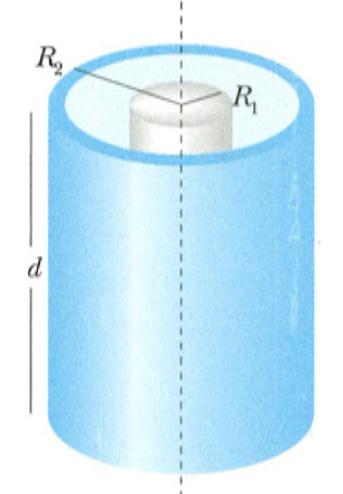
\includegraphics[scale=0.4]{condensatore_cilindrico.png}
    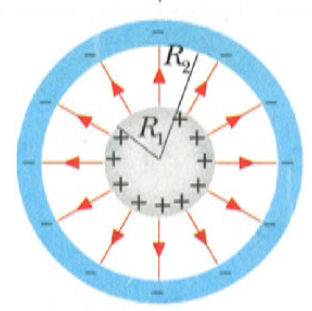
\includegraphics[scale=0.6]{condensatore_cilindrico_sezione.png}
    \centering
    \caption{}
\end{figure}

con \(\Sigma = 2 \pi R d\) area delle armature distanti \(h\): ritrovo (\ref{capacita_condensatore})

Da \ref{capacita_condensatre_cilindrico} definisco la \emph{capacità per unità di lunghezza}
\begin{equation}
    C_d = \frac{C}{d} = \frac{2 \pi \epsilon_0}{\ln \frac{R_2}{R_1}}
\end{equation}

\subsection{Capacità di un condensatore piano}

Le armature di un condensatore piano sono costituite da due conduttori piani paralleli, di area \(\Sigma\) e distanti \(h\).
La carica positiva \(q\) è distribuita con densità uniforme a sull'armatura positiva e quella negativa \(- q\) con densità uniforme \(-\sigma\) sull'armatura negativa. 

La capacità di un condensatore piano è data da 
\begin{equation}
    C = \frac{q}{V_1 - V_2} = \frac{\epsilon_0 \Sigma}{h}
\end{equation}

\begin{figure}[h]
    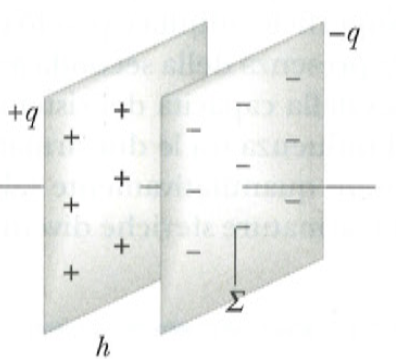
\includegraphics[scale=0.4]{condensatore_piano.png}
    \centering
    \caption{}
\end{figure}

Questa volta non ci sono approssimazioni geometriche, però quest'ultima è approssimata per un'altra ragione: il campo si può supporre uniforme solo nella regione centrale del condensatore, lontano dai bordi.

\section{Collegamento di condensatori}

Un condensatore viene utilizzato essenzialmente come deposito di carica; pur essendo la carica totale nulla, essa è separata nella quantità \(+q\) e \(-q\), proporzionali per un conduttore di data capacità alla differenza di potenziale tra le armature.
Tramite opportuni collegamenti conduttivi esterni è possibile far fluire la carica negativa ( elettroni) da un'armatura all'altra, generando una corrente elettrica che scarica il condensatore. 

Possiamo però subito descrivere come si collegano con fili conduttori più condensatori tra loro e calcolare la capacità equivalente. 
Noi supponiamo costanti nel tempo le cariche e le differenze di potenziale, però i risultati sono validi anche in regime variabile.

\subsection{Condensatori in parallelo}

La connessione in parallelo delle armature consiste nel realizzare due soli conduttori. 
In tal modo, essendo ciascun conduttore equipotenziale, la \(d.d.p.\) applicata al condensatore \(C_1\) è eguale a quella applicata al condensatore \(C_2\).
\begin{equation*}
    q_1 = C_1 V \ , \ q_2 = C_2 V
\end{equation*}
La carica globale sul conduttore superiore, costituito dalle due armature superiori è
\begin{equation*}
    q = q_1 + q_2 = \left(C_1 + C_2 \right)V
\end{equation*}
sul conduttore inferiore la carica è \(-q = -( q_1 + q_2)\). Definiamo capacità equivalente del sistema
\begin{equation}
    C_{eq} = \frac{q}{V} = C_1 + C_2
\end{equation} 

Due condensatori in parallelo si comportano come un unico condensatore la cui capacità è data dalla somma delle capacità dei componenti. 
Il ragionamento si estende a \(n\) condensatori:
\begin{equation*}
    C_{eq} = C_1 + ... + C_n
\end{equation*}
\emph{in un sistema di condensatori in parallelo ai capi di ciascuno c'è la stessa differenza di potenziale e la capacità equivalente è somma delle singole capacità}.

\subsection{Condensatori in serie}

Nella connessione in serie c'è un solo collegamento tra i due condensatori e viene costituito un sistema composto da \(n\) conduttori: ai due estremi si applica la differenza di potenziale \(V = V_C-V_A\) e il conduttore intermedio assume un potenziale \(V_B\).
Se \(+q\) è la carica sull'armatura di \(C_1\) a potenziale \(V_C\), per induzione compare la carica \(-q\) sull'armatura affacciata e \(+q\) sull'armatura di \(C_2\) a questa collegata, dovendo essere il conduttore centrale neutro; sempre per induzione compare la carica \(-q\) sull'armatura di \(C_2\) a potenziale \(V_A\). 
Vediamo che il valore della carica è lo stesso nei due condensatori. 
\begin{equation*}
    V_C -V_B = \frac{q}{C_1} \ , \ V_B - V_A = \frac{q}{C_2}
\end{equation*}
\begin{equation*}
    V = V_C -V_B = \frac{q}{C_1} + \frac{q}{C_2} = q \left(\frac{1}{C_1} + \frac{1}{C_2}\right) = \frac{q}{C_{eq}}
\end{equation*}
\begin{equation*}
    \frac{1}{C_{eq}} = \frac{1}{C_1} + \frac{1}{C_2} , \ , C_{eq} = \frac{C_1 C_2}{C_1 + C_2}
\end{equation*}

Il ragionamento si estende a \(n\) condensatori:
\begin{equation}
    \frac{1}{C_{eq}} =  \frac{1}{C_{1}} +  \frac{1}{C_{2}} + ... +  \frac{1}{C_n}
\end{equation}

\emph{in un sistema di condensatori in serie la carica è la stessa su ciascuno, l'inverso della capacità equivalente è somma degli inversi delle singole capacità}. 

\section{Energia del campo elettrico}

\subsection{Carica di un condensatore}

Il processo di carica di un condensatore, in cui si passa dalla situazione di carica zero sulle armature alla situazione ( \(+q\), \(-q\)) con una differenza di potenziale \(V =q / C\) tra le armature, consiste in definitiva in una separazione di cariche e richiede un determinato lavoro che, essendo il campo elettrostatico conservativo, dipende soltanto dallo stato iniziale e dallo stato finale.
Per eseguire il calcolo possiamo immaginare quindi che la carica di un condensatore avvenga sottraendo, tramite un agente esterno, una carica \(dq\) dall'armatura negativa e portandola sull'armatura positiva, così che alla fine una carica \(+q\) è stata trasferita da un'armatura all'altra, lasciando la prima con una carica \(-q\), e si è stabilita tra le armature la differenza di potenziale \(V\); la carica totale è in ogni istante nulla.

Se in una fase intermedia del processo la differenza di potenziale tra le armature è \(V^{\prime}\), in quanto è già stata trasferita la carica \(q' = C V^{\prime}\) il lavoro per spostare l'ulteriore carica \(dq^{\prime}\) attraverso la differenza di potenziale \(V^{\prime}\) è
\begin{equation*}
    d W = V^{\prime} d q^{\prime} = \frac{q^{\prime}}{C} d q^{\prime}
\end{equation*}
e quindi il valoro complessivo per effettuare la separazione delle cariche è
\begin{equation*}
    W = \int dW = \int_0^q \frac{q^{\prime}}{C}d q^{\prime} = \frac{q^2}{2 C}
\end{equation*}
Esso dipende solo dalla carica trasportata e dalla capacità del condensatore e non contiene informazioni sul processo effettivo.

Questo lavoro, effettuato contro la forza elettrostatica che si oppone a un accumulo di cariche dello stesso segno, viene immagazzinato nel sistema sotto forma di energia (potenziale) elettrostatica. 
Assumendo che l'energia sia nulla quando \(q = 0\), abbiamo \(W = U_e\), servendoci delle ( \ref{capacita_condensatore}), scriviamo tre espressioni equivalenti per l'energia elettrostatica del condensatore di capacità \(C\), carico con carica \(q\) e differenza di potenziale \(V\):
\begin{equation} \label{energia_elettrostatica}
    U_e = \frac{1}{2} \frac{q^2}{C} = \frac{1}{2} C V^2 = \frac{1}{2} q V
\end{equation} 

Alle stesse espressioni si arriva per l'energia elettrostatica di un conduttore carico isolato immaginando il processo di carica come un trasporto di carica dall'infinito, dove \(V = 0\), alla superficie del conduttore. 
Ciò torna formalmente con l'idea di considerare un conduttore isolato come un condensatore con un'armatura all'infinito.

Il ragionamento svolto per il calcolo dell'energia del condensatore lega l'energia alle cariche, che la possiedono in quanto si trovano ad un certo potenziale: l'energia totale è la somma delle energie potenziali delle singole cariche. 
È però possibile trovare un'espressione alternativa dell'energia, legata al campo elettrostatico prodotto dal sistema di cariche piuttosto che alle sorgenti del campo stesso.
Riprendo (\ref{energia_elettrostatica}) con la relazione \(V =Eh\)
\begin{equation*}
    U_e = \frac{1}{2} C V^2 = \frac{1}{2} \frac{\epsilon_0 \Sigma}{h} E^2 h^2 = \frac{1}{2} \epsilon_0 E^2 \Sigma h = \frac{1}{2} \epsilon_0 E^2 \tau
\end{equation*}
essendo \(\tau = \Sigma h\) il volume del condensatore, cioè il volume in cui è definito il campo elettrostatico.

Se facciamo l'ipotesi che l'energia elettrostatica sia distribuita nei punti in cui c'è campo elettrostatico e che questa distribuzione sia uniforme come il campo, possiamo dire che la densità di energia elettrostatica, ovvero l'energia elettrostatica per unità di volume, è
\begin{equation} \label{densita_energia_elettrostatica}
    u_e = \frac{U_e}{\tau} = \frac{1}{2} \epsilon_0 E^2
\end{equation}
che risulta pertanto \emph{proporzionale al quadrato del campo elettrostatico}.  
La generalità di questa formula, in cui non compare alcun elemento caratteristico del sistema per cui il calcolo è stato eseguito, ma soltanto il valore del campo e una proprietà del mezzo (in questo caso il vuoto), suggerisce che (\ref{densita_energia_elettrostatica}) si possa applicare a qualsiasi situazione.

In effetti si può dimostrare che in una regione in cui è definito un campo elettrostatico l'energia contenuta in ogni volume infinitesimo \(d \tau\), al cui interno il campo elettrostatico vale \(E\) è 
\begin{equation*}
    d U_e = u_e d \tau = \frac{1}{2} \epsilon_0 E^2 d \tau
\end{equation*}
l'energia totale del campo elettrostatico si ottiene integrando su tutto il volume in cui il campo elettrostatico è diverso da zero: 
\begin{equation} \label{energia_totale_campo_elettrostatico}
    U_e = \int d U_e = \int \frac{1}{2} \epsilon_0 E^2 d \tau
\end{equation}
Questa energia corrisponde al lavoro speso per costruire la distribuzione di cariche che dà origine al campo elettrostatico. 
Le (\ref{densita_energia_elettrostatica}) e  (\ref{energia_totale_campo_elettrostatico}) valgono per qualsiasi campo elettrico, indipendentemente dalla sua natura.

\subsection{Pressione elettrostatica}

Calcolo la forza tra due armature di un condensatore piano, di area \(\Sigma\) distanti \(h\), carico con una carica \(q\), e il rapporto \(F/\Sigma\), detto pressione elettrostatica.  
L'energia elettrostatica di un condensatore piano con armature di area \(\Sigma\) distanti \(h\) è: 
\begin{equation*}
    U_e = \frac{q^2}{2 C} = \frac{q^2}{2 \epsilon_0 \Sigma} h
\end{equation*}

Tra le armature, cariche di segno opposto, si esercita una forza \(F\) attrattiva che per ragioni di simmetria è parallela a \(\overrightarrow{E}\).  
Per uno spostamento \(dh\) dell'armatura positiva ( \(dh < 0\)) l'energia elettrostatica diminuisce di
\begin{equation*}
    d U_e = \frac{q^2}{2 \epsilon_0 \Sigma} dh = \frac{\sigma^2}{2 \epsilon_0}  \Sigma dh
\end{equation*}
e viene fornito dalla forza \(\overrightarrow{F}\) il lavoro
\begin{equation*}
    d W = \overrightarrow{F} \cdot d \overrightarrow{h} = - d U_e = - \frac{q^2}{2 \epsilon_0} \Sigma dh > 0
\end{equation*}
positivo, per cui la forza \(\overrightarrow{F}\) è concorde a \(dh\) e vale:
\begin{equation}
    F =  - \frac{\sigma}{2 \epsilon_0} \Sigma 
\end{equation}

Esprimendo \(\sigma\) in funzione del campo elettrostatico \(E\) abbiamo in modulo:
\begin{equation*}
    F =  - \frac{\sigma}{2 \epsilon_0} \Sigma = \frac{1}{2} \epsilon_0 E^2 \Sigma
\end{equation*}
e la forza per unità di superficie risulta 
\begin{equation} \label{pressione_elettrostatica}
    p_{el} = \frac{F}{\Sigma} = \frac{1}{2} \epsilon_0 E^2
\end{equation} 
detto \emph{pressione elettrostatica}.

La (\ref{pressione_elettrostatica}), che non contiene elementi caratteristici del sistema (anche forma del condensatore), ha validità generale, qualsiasi sia la distribuzione di carica superficiale e mostra che la pressione elettrostatica ha la stessa espressione della densità di energia. 

\subsubsection*{Pressione elettrostatica in condensatore isolato}

In un condensatore isolato vale:
\begin{equation*}
    Q = \text{costante} \implies \sigma = \frac{Q}{\Sigma} = \text{costante} \implies E = \frac{\sigma}{\epsilon_0} = \text{costante}
\end{equation*}
Ottengo quindi
\begin{equation*}
    F = - \frac{d}{dh} \left[\frac{1}{2} \epsilon_0 E^2 S h\right] = - \frac{1}{2} \epsilon_0 E^2 S
\end{equation*}
pertanto la pressione elettrostatica sarà:
\begin{equation*}
    p_{el} = - \frac{1}{2} \epsilon_0 E^2
\end{equation*}

\subsubsection*{Pressione elettrostatica in condensatore attaccato ad un generatore}

In un condensatore isolato vale:
\begin{equation*}
    \Delta V = \text{costante}
\end{equation*}
dato che \(C = \frac{Q}{\Delta V}\) ottengo che:
\begin{equation*}
    \Delta V = \frac{Q}{C} = \text{costante}
\end{equation*} 
Per trovare la forza devo misurare la variazione dell'energia del generatore e del condensatore stesso:
\begin{equation*}
    \Delta U_{TOT} = \Delta U_{GEN} + \Delta U_{el}
\end{equation*}
dove \(\Delta U_{GEN}\) carica energia nel condensatore.\newline 
Varia la capacità e quindi varia anche la carica, quindi vale:
\begin{equation*}
    q^{\prime} - q  = \left(C^{\prime }- C\right) \Delta V = \epsilon_0 S \left(\frac{1}{h-dh} + \frac{1}{h}\right) \Delta V
\end{equation*}
\begin{equation*}
    q^{\prime} - q  = \frac {\epsilon_0 S}{h} \Delta V dh 
\end{equation*}
Il lavoro del generatore è quindi
\begin{equation*}
    W_{GEN} = \left(q^{\prime} - q\right) \Delta V = \epsilon_0 S dh \left(\frac{\Delta V }{h}\right)^2 
\end{equation*}
La differenza di energia elettrostatica del condensatore sarà quindi:
\begin{equation*}
    d \left(\Delta U_{el}\right) = - \frac{1}{2} \epsilon_0 \left(\frac{\Delta V}{h}\right)^2 S dh 
\end{equation*}
La differenza di energia elettrostatica del generatore sarà quindi:
\begin{equation*}
    d \left(\Delta U_{gen}\right) = - \frac{1}{2} \epsilon_0 \left(\frac{\Delta V}{h}\right)^2 S dh 
\end{equation*}
La variazione totale è:
\begin{equation*}
    d \left(\Delta U\right) = \frac{1}{2} \epsilon_0 \left(\frac{\Delta V}{h}\right)^2 S dh 
\end{equation*}
La forza diventa:
\begin{equation*}
    F = - \frac{d \Delta U }{dh} =  - \frac{1}{2} \epsilon_0 \left(\frac{\Delta V}{h}\right)^2 S
\end{equation*}
dato \(\left(\frac{\Delta V}{h}\right)^2 = E^2\) la pressione elettrostatica è come stabilito precedentemente:
\begin{equation*}
    p_{el} = - \frac{1}{2} \epsilon_0 E^2
\end{equation*}

\end{document}
